 \let\negmedspace\undefined
\let\negthickspace\undefined
\documentclass[journal]{IEEEtran}
\usepackage[a5paper, margin=10mm, onecolumn]{geometry}
%\usepackage{lmodern} % Ensure lmodern is loaded for pdflatex
\usepackage{tfrupee} % Include tfrupee package

\setlength{\headheight}{1cm} % Set the height of the header box
\setlength{\headsep}{0mm}     % Set the distance between the header box and the top of the text

\usepackage{gvv-book}
\usepackage{gvv}
\usepackage{cite}
\usepackage{amsmath,amssymb,amsfonts,amsthm}
\usepackage{algorithmic}
\usepackage{graphicx}
\usepackage{textcomp}
\usepackage{xcolor}
\usepackage{txfonts}
\usepackage{newtxtext,newtxmath}
\usepackage{listings}
\usepackage{enumitem}
\usepackage{mathtools}
\usepackage{gensymb}
\usepackage{comment}
\usepackage[breaklinks=true]{hyperref}
\usepackage{tkz-euclide} 
\usepackage{listings}
% \usepackage{gvv}                                        
\def\inputGnumericTable{}                                 
\usepackage[latin1]{inputenc}                                
\usepackage{color}                                            
\usepackage{array}                                            
\usepackage{longtable}                                       
\usepackage{calc}                                             
\usepackage{multirow}                                         
\usepackage{hhline}                                           
\usepackage{ifthen}                                           
\usepackage{lscape}

\begin{document}

\bibliographystyle{IEEEtran}
\vspace{3cm}

\title{1.10.24}
\author{EE25BTECH11058 - Tangellapalli Mohana Krishna Sushma}
% \maketitle
% \newpage
% \bigskip
{\let\newpage\relax\maketitle}

\renewcommand{\thefigure}{\theenumi}
\renewcommand{\thetable}{\theenumi}
\setlength{\intextsep}{10pt} % Space between text and floats
\textbf{Question}:
 Find the direction cosines of the unit vector perpendicular to the plane
\begin{align*}
    \vec{r} \cdot (6\hat{\imath} - 3\hat{\jmath} - 2\hat{k}) + 1 = 0
\end{align*}
\hspace{1cm}passing through the origin.
\bigskip

\textbf{Solution}:

\vspace{8pt}

Given:

\vspace{8pt}

Plane equation, 
\begin{align}
    \vec{r} \cdot (6\hat{i} - 3\hat{j} - 2\hat{k}) + 1 = 0 
\end{align}

Let the unit vector perpendicular to the plane passing through the origin be $\vec{u}$.

From above,

The plane's normal vector,
\begin{align}
    \vec{n} = 
    \begin{pmatrix}
        6 \\
        -3 \\
        -2
    \end{pmatrix}
\end{align}

Norm of the vector $\vec{n}$,
\begin{align}
    \vec{u} = \frac{1}{\|\vec{n}\|} \vec{n} 
    = \frac{1}{7}
    \begin{pmatrix}
        6 \\[2pt]
        -3 \\[2pt]
        -2
    \end{pmatrix}
    =
    \begin{pmatrix}
        \dfrac{6}{7} \\[2pt]
        -\dfrac{3}{7} \\[2pt]
        -\dfrac{2}{7}
    \end{pmatrix}
\end{align}


The direction cosines of the unit vector perpendicular to the plane are 
\[
    \left(
        \frac{6}{7},\;
        -\frac{3}{7},\;
        -\frac{2}{7}
    \right)
\]

\begin{figure}
    \centering
    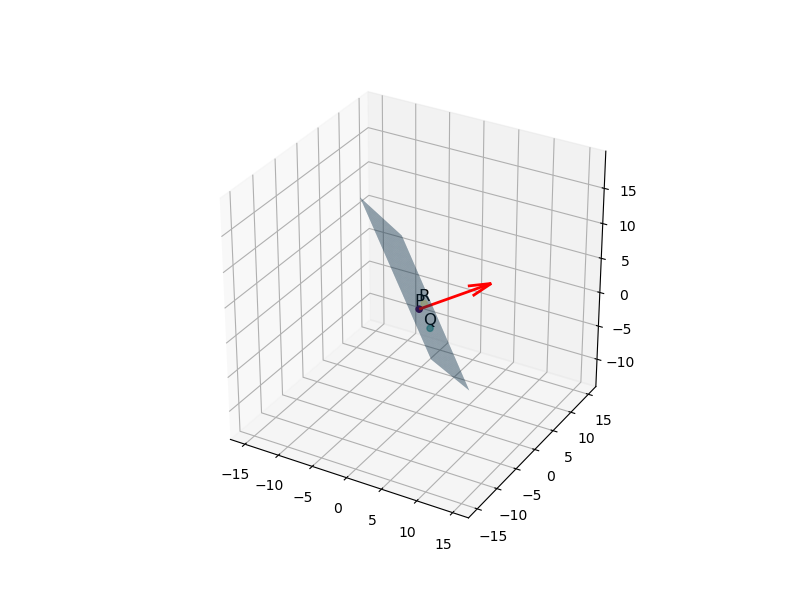
\includegraphics[width=0.8\columnwidth]{figs/fig.png}
    \caption{Plane with Perpendicular Normal Vector}
    \label{fig:placeholder}
\end{figure}

\end{document}